\documentclass[parskip=half,german]{scrartcl}

\usepackage[ngerman]{babel}
\usepackage[utf8]{inputenc}
\usepackage{microtype}
\usepackage{graphicx}

\title{Konkretisierung der Zielstellung für die Kooperation}
\subtitle{}
\author{Jonas Sternisko}



\begin{document}
  \maketitle

  \begin{abstract}
% Was steht in diesem Text?  
Dieses Dokument beschreibt die Problemstellung und die daraus abgeleitete
Aufgabenstellung für den Kooperationsvertrag, wie sie die Arbeitsgruppe vom
Lehrstuhl für Algorithmen und Datenstrukturen (im Folgenden AD genannt) aus den
bisherigen Treffen aufgefasst hat. Es definiert ein Modul für das
Geoinformationssystem (GIS) als Arbeitsziel, welches die Simulation der
Benutzung vom Waldwegen zu Erholungszwecken in annehmbarer Zeit ermöglicht.
Dieses Hauptziel wird anschließend in teilweise aufeinander aufbauende
Meilensteine untergliedert.
% Warum ist das notwenig? --> Verwirrung durch unpräzise Problembeschreibung
% Nutzen des Dokuments
Dieser Text soll etwaige Mißverständnisse in der Kommunikation zwischen FVA
(Forstwissenschaftler) und AD (Informatiker) aufdecken und verhindern helfen.
Gleichzeitig dient er als Arbeitsgrundlage für die Algorithmenentwicklung.
  \end{abstract}

  
\section{Problembeschreibung}
Ausgehend von Daten über die Siedlungsverteilung und über die Nutzung des Waldes
zur Erholung soll ein Benutzungsmodell für Waldwege erstellt werden.
Die Besucheranzahl von Wäldern hängt von deren Lage ab. Die Anzahl von Menschen,
die den Wald innerhalb akzeptabler Zeit mit Hilfe verschiedener Verkehrsmitteln
erreichen können, ist hier entscheidend.
Innerhalb des Waldes bewegen sich Besucher überwiegend auf Waldwegen. Um die
Benutzung des Waldes zu simulieren, bedarf es eines Modells für die Benutzung
der Waldwege. Daraus lässt sich schließen, ob und wie stark ein Waldstück
besucht wird.

  
\section{Algorithmus}
\subsection{Überblick}
% Bevölkerung -> WEP -> Touren -> Modell für die Benutzungshäufigkeit der   
% Wege im Wald
Aus Daten über die Siedlungsverteilung und die Erholungsgewohnheiten der
Bevölkerung wird zunächst berechnet, welche Wälder für jeden Siedlungsraum
erreichbar sind und an welchen Stellen die Menschen den Wald betreten.
Ausgehend von diesen Orten werden plausible Routen durch den Wald simuliert.
Diese werden nach ihrer Attraktivität gewichtet. In der Summe ergibt sich für
jeden Wegabschnitt, wie viele Menschen diesen Weg benutzen.

\subsection{Detail}
Als \emph{Siedlungsfläche} bezeichnen wir grob gesagt alle Areale, in denen sich
eine hinreichend große Anzahl von Wohnhäusern oder Unterkünften (Hotels,
Pensionen etc.) befindet. Die Siedlungsfläche muss nicht unbedingt mit der
Gemeindefläche übereinstimmen. So ist es vorstellbar, dass man für eine
Verfeierung des Models zum Beispiel Wohngegenden von Gewerbegebieten
anhand von OSM-Daten unterscheidet.

Als \emph{Waldeinstiegspunkte} (WEP) bezeichnen wir Orte, an denen Wege den
Waldrand überschreiten. Mathematisch gesehen sind dies Schnittpunkte von Kanten
des Wegenetzes mit den Kanten des den Wald begrenzenden Polygons. Darüber hinaus
können besondere Orte wie zum Beispiel Parkplätze Waldeinstiegspunkte
darstellen. 
    
      
\subsection*{Frequentierung von Waldeinstiegspunkten}
Touren, die im Wald zurückgelegt werden beginnen und enden an (möglicherweise
verschiedenen) WEPs. Wie viele Menschen an einem WEP den Wald betreten (oder
wieder verlassen) hängt von dessen Lage gegenüber der umgebenden
Siedlungsgebieten und der Mobilität der dortigen Bevölkerung ab. Durch
Bevölkerungsstatistiken ist die Populationsverteilung bekannt und die Umfragen
seitens der FVA geben Aufschluss über die \emph{Erhohlungsmobilität} zu Fuss,
mit dem Fahrrad oder mit dem Auto.

Ausgehend von den durch die FVA bereit gestellten Daten über
Bevölkerungsverteilung in den Siedlungsgebieten und deren Erholungsmobilität
wird in einem ersten Schritt die Frequentierung der WEPs berechnet. Das heißt,
welcher Anteil der Bevölkerungauf jeden WEP entfällt.

Algorithmisch könnte man dies durch die Berechnung des minimalen Spannbaums
von jedem WEP auf dem Straßennetz umsetzen (für verschiedene
Maximalgeschwindigkeiten). Dabei wird die Siedlungsfläche in hinreichend große
Parzellen unterteilt. Das Gewicht eines WEP errechnet sich dann aus der Anzahl
Personen, für welche dieser WEP erreichbar ist, gewichtet mit der Anzahl
erreichbarer WEPs für die jeweilige Parzelle und der Distanz zwischen WEP und
Parzelle.


\subsection*{Simulation von Touren im Wald}
Im Wald zu Erholungszwecken zurückgelegte Strecken haben verschiedene
Charackteristika. Es werden in der Regel Touren bevorzugt, die nahe an
verschiedenen Attraktoren (Aussichtspunkte, Gasthöfe, Gewässer, \dots)
verlaufen und bei denen keine Orte mehrmals besucht werden.
Die Länge der Touren und das Steigungsprofil hängt von den Präferenzen der
Wanderer ab. Laut den Ergebnissen der FVA sind rund 80\% aller Touren Rundwege,
d.h. sie kehren zum Startpunkt zurück.

Um die von einem WEP ausgehenden Touren zu modellieren, ist die einfachste
Lösung eine Aufzählung aller möglichen Wege. Da die Länge der Wege beschränkt
und der durch die Waldwege beschriebene Graph \emph{sparse} ist (d.h. von jedem
Ort im Wald gibt es nur wenige weiterführende Wege), könnte dies schon eine
ausreichend schnelle Lösung des Problems darstellen. Andernfalls müsste hierfür
eine geeignete Beschleunigungsmethode gefunden oder neu entwickelt werden. 
Die so ermittelten Touren werden anhand ihres Profils gewertet (Kriterien
siehe oben). Zusammen mit dem Gewicht des WEP ergibt sich ein Model, wie häufig
diese Tour benutzt wird. Ein Model für alle Waldwege ergibt sich durch
Summierung über die einzelnen Teilstrecken aller Touren von allen WEPs.

\subsection*{Vereinfachungen}
Um die Rechenzeit der Simulation in einem sinnvollen Rahmen zu halten, werden
verschiedene Vereinfachungen vorgenommen. Im bestehenden GIS-Modul wurde die
Simulation zum Beispiel auf einzelne Landkreise beschränkt und die
Siedlungsfläche auf Punkte in einem gleichmäßigen Gitter mit 500\,m Auflösung
heruntergebrochen. Weil oftmals auch Ziele außerhalb des eigenen Landkreises
besucht werden, ist dies eine sehr starke Vereinfachung. Wir sind zum jetzigen
Zeitpunkt optimistisch, dass durch geeignete Algorithmen die Simulation auch auf
Landesebene mit einer feineren Auflösung in sinnvoller Zeit möglich wird. 

% Geschwindigkeit im Wald (bei Steigung, Wegetyp, ...)
Weitere mögliche Vereinfachungen, welche die Rechenzeit reduzieren, ohne dass
das Modell zu einfach wird, sind zum Beispiel die Annahme konstanter
Laufgeschwindigkeiten auf Waldwegen unabhängig von der Steigung und ...

% Konstante Geschwindigkeit im Wald annehmen. Eventuell ungerichtete Kanten
% durch zwei gerichtete ersetzen. Geschwindigkeit dieser richtet sich nach
% Steigung.
    
  
\section{GIS-Modul}
Ziel des Projekts ist ein Modul für das von der FVA eingesetzte Programm ArcGIS.
Dieses verfügt über eine Python-Programmierschnittstelle (ArcPy). Die
Implementierung seitens AD erfolgt in C++, denn diese Programmiersprache is am
besten geeignet, Geschwindigkeit und Speicherverbrauch der Simulation zu
optimieren. 

Nach jetzigem Kenntnisstand ist die einfachste Lösung für diese Schnittstellen
ein Python-Modul (Wrapper-Module) für ArcPy, welches ein weiteres Modul
(Extension-Module, w.g. Python-Extension) aufruft. Das Wrapper-Modul
übernimmt die Aufgaben, die Daten und Parameter aus dem GIS in eine geeignete
Form für das interne Modul zu bringen und nach Abschluss der Simulation deren
Ergebnisse in ein für das GIS verwertbares Format zu überführen. Das
Extension-Modul ruft den C++-Code auf.

\begin{figure}
  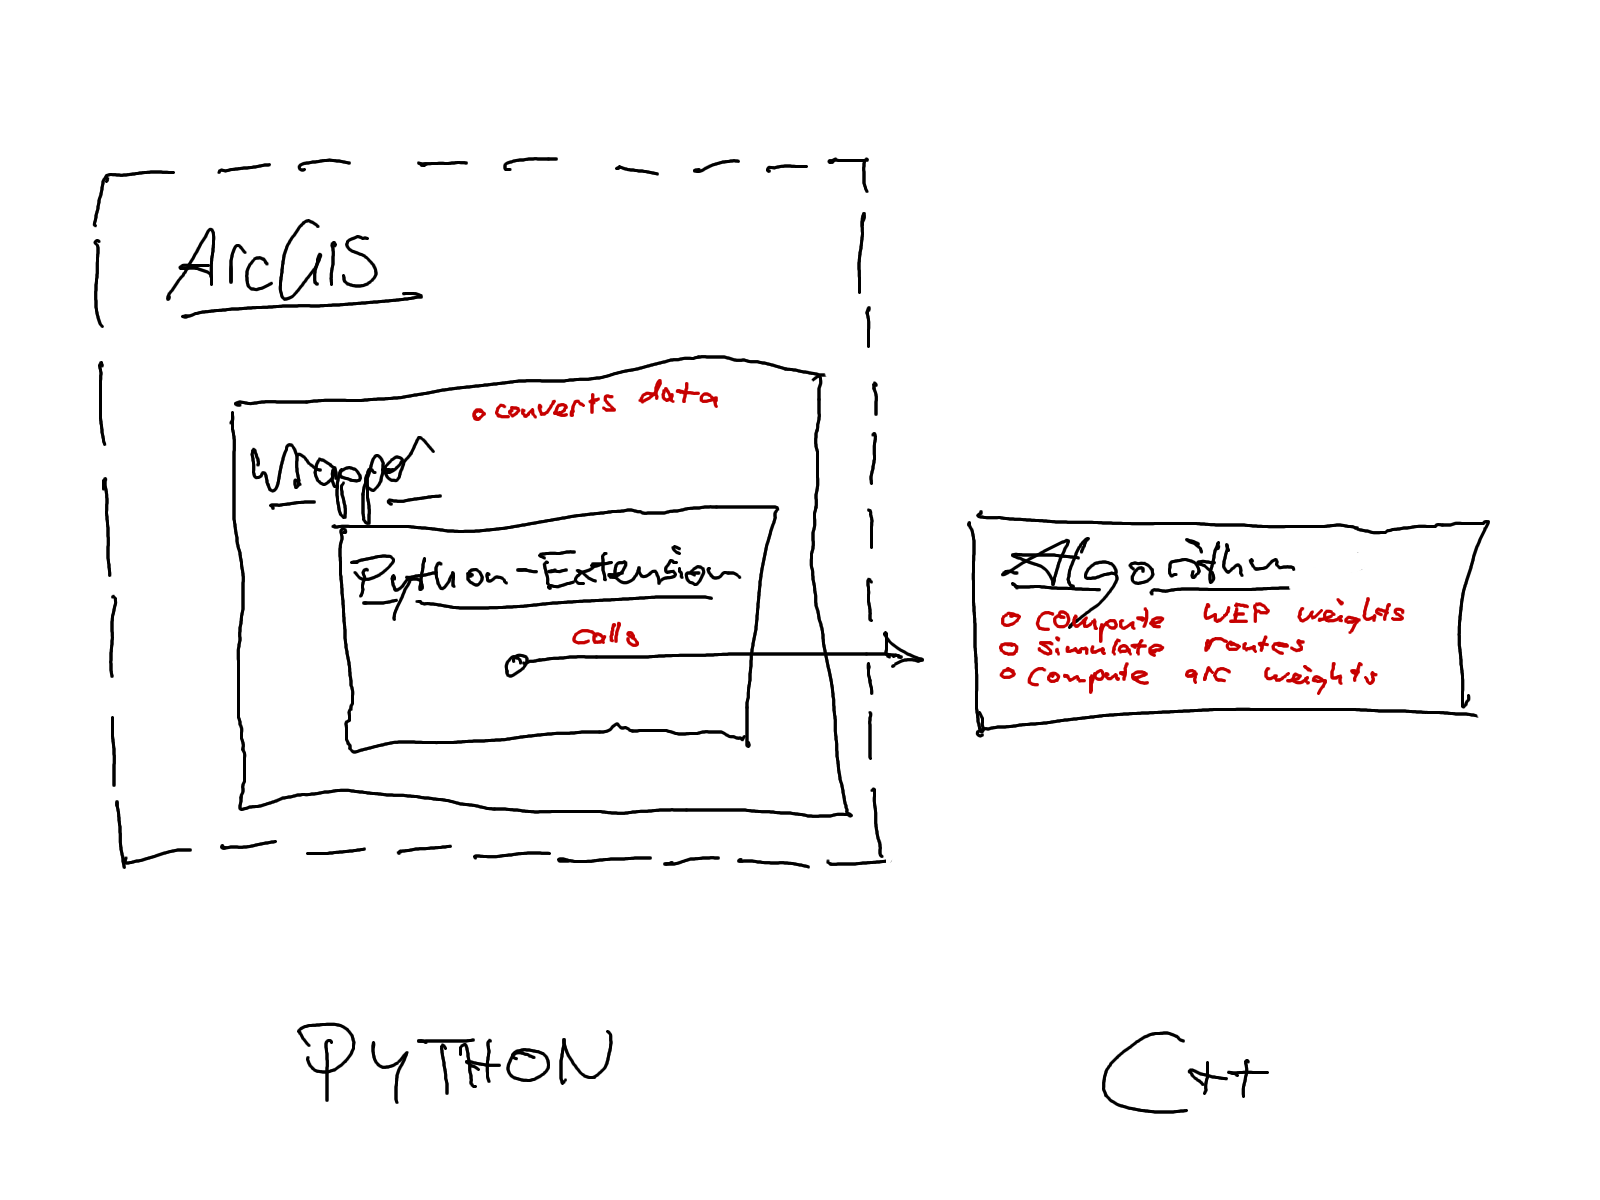
\includegraphics[width=\textwidth]{UML.png}
  \caption{Zu entwickelnde Komponenten}
\end{figure}

\subsection*{Eingabe}
     Graph information
     \begin{itemize}
      \item Roadnetwork including forest tracks (separated?)
      \item Forestal areas (as polygons)
      \item Forest entry points (set of coordinates or node IDs)
      \item Set of attractors 
     \end{itemize}
     
     Population and mobility information
     \begin{itemize}
      \item Populated areas (as polygons?) with population count
      \item Survey results 
        \begin{itemize}
         \item Means and range of mobility
         \item Key data on routes in the forest (preferred distance, maximum
slope, ...)
        \end{itemize}

     \end{itemize}


    
\subsection*{Ausgabe}
     \begin{itemize}
      \item Liste mit Paaren aus Waldweg-ID und berechnetem Gewicht
     \end{itemize}


    
\subsection*{Parameter}
\begin{itemize}
 \item Auflösung Gitter
 \item ...
\end{itemize}
      
      
  
\end{document}

% Idee: Partikelfilter für Routengenerierung.

% Frage: Begrifflichkeiten besser in Englisch benutzen?